\chapter{Apprentissage Machine d'Architectures Profondes}


\section{Introduction à l'Apprentissage Statistique}

L'apprentissage machine est un champ de recherche de l'intelligence
artificielle. Il permet notamment d'extraire des informations utiles à l'aide à
la décision.  L'objectif ici est de pouvoir extraire de manière quasiment
automatique à partir de grandes masses de données une information pertinente.
C'est l'immense quantité de données (ou leur dimensionnalité trop élevée)  qui
rend cette tâche difficile, parfois impossible, à accomplir pour un être
humain.

\section{Applications de cette thèse}

Les chercheurs en apprentissage machine résolvent une grande variété de
problèmes sitôt qu'un ensemble suffisant de données est disponible. Dans ce
travail, on considère les tâches suivantes:
\\

\begin{itemize}

\item {\bf Apprentissage de représentation non supervisé.} L'ensemble de
données ne contient pas de labels, seulement des entrées $x\in\mathbb{R}^{d}$.
L'objectif est d'apprendre une représentation des données $h(x)$ de meilleure
qualité que la représentation brute $x$.  Ces qualités vont de la réduction de
dimensionnalité (Chapitres~\ref{chap:utlc}, \ref{chap:ob}), une meilleure
séparabilité linéaire (Chapitres~\ref{chap:utlc}, \ref{chap:ob}), de meilleures
propriétés de mixage (Chapitre~\ref{chap:mixing}) ou une meilleure
initialisation des paramètes pour un apprentissage supervisé
(Chapitre~\ref{chap:ob}). 
\\

\item {\bf Transfert de domaine.} Le résultat de l'algorithme est utilisé sur
un ensemble de données cible $\tilde{\mathcal{D}}$ autre que l'ensemble
d'entraînement $\mathcal{D}$. Cela permet d'avoir une représentation plus
spécifique à l'ensemble cible tout en obtenant un gain de performances dû par
exemple, à l'utilisation d'un plus grand ensemble de données d'entraînement.
Dans ce travail, nous présenterons l'utilisation d'un proxy d'apprentissage
(Chapitre~\ref{chap:mlj}), d'une PCA transductive (Chapitre~\ref{chap:utlc}) et
d'un fine-tuning sur l'ensemble cible (Chapitre~\ref{chap:ob}).
\\

\item {\bf Apprentissage d'espaces sémantiques multi-domaines.} L'idée ici est
d'avoir une représentation vectorielle dans un espace euclidien pour chaque entité. Un
$mot$ est associé à un vecteur $x_{mot}\in\mathbb{R}^{d}$ qui est ajusté lors de l'apprentissage.
Ces espaces possèdent une sémantique propre dans le sens où des vecteurs proches
dans cet espace ont un sens similaire. Par exemple des mots voisins vont avoir
la même syntaxe (ex: adjectif, nom) ou une sémantique proche (ex: pays, mesure).
Nous montrerons qu'il est possible d'avoir un espace commun à plusieurs domaines
comme des mots et des images (Chapitre~\ref{chap:mlj}).
\\

\item {\bf Classification de séquences.} Il s'agit ici de classifier des
données $x_{t}$ qui en plus d'avoir un label $y_{t}$, possèdent une composante
temporelle. Ceci est un aspect du problème intéressant à exploiter du fait des
dépendances possibles entre les prédictions à $t-1$, $t$ et $t+1$ par exemple.
Des architectures spécifiques de type RNN pour l'apprentissage d'un espace
sémantique modélisant le contexte seront présentées ici
(Chapitre~\ref{chap:rnn}).

\end{itemize}

\section{Risque Empirique et Espéré}

Commençons d'abord par une formalisation du problème d'apprentissage.
L'objectif est de trouver une fonction $f\in\mathcal{F}$ qui va exécuter une
tâche particulière. Il faut donc définir l'espace des fonctions $\mathcal{F}$
parmi lequel nous allons chercher la solution optimale à notre problème.  Il
faut également définir une fonction de coût ou d'objectif $\mathcal{C}$ qui
évalue retourne un réél $\mathcal{C}(\mathcal{D},f)\in\mathbb{R}$ nous
permettant d'évaluer la qualité d'une fonction donnée sur un échantillon de
données $\mathcal{D}$.

La solution à notre problème est donc la fonction $f^*$ définie par:

\begin{equation}
\label{eq:graal}
f^* = \argmin_{f \in \mathcal{F}} {\mathbb E}_\mathcal{D}[\mathcal{C}(\mathcal{D},f)]
\end{equation}


En supposant qu'on ait accès à une infinité de données, nous serions en mesure
de calculer de façon exacte le {\bf risque espéré} ${\mathbb
E}_\mathcal{D}[\mathcal{C}(\mathcal{D},f)]$. Malheureusement, l'ensemble de
données $\mathcal{D}$ est de taille finie et on ne peut disposer que d'un estimé
du risque espéré. L'idée est de minimiser l'objectif sur un ensemble d'entraînement
$\mathcal{C}(\mathcal{D}_\textrm{train},f)$ puis d'approximer le risque espéré sur un ensemble
qui n'a pas été vu lors de l'apprentissage, un ensemble de test
$\mathcal{D}_\textrm{test}$. On va donc minimiser le {\bf risque empirique} sur
l'ensemble d'entraînement:

\begin{equation}
\label{eq:graal}
\hat{f}^* = \argmin_{f \in \mathcal{F}} \mathcal{C}(\mathcal{D}_\textrm{train},f)]
\end{equation}

Pour une quantité de données limitée, il est possible de trouver une fonction
$f\in\mathcal{F}$ qui donne un risque empirique proche de $0$ pourvu que
$\mathcal{F}$ définisse un espace de fonctions à la complexité assez élevée (il
est parfois possible de mesurer cette complexité avec la dimension de
Vapnik-Chervonenkis~\citep{Vapnik71}). Mais ceci ne résulte pas nécessairement en une solution
qui généralise bien sur de nouvelles données qui n'ont pas été utilisées au
cours de l'entraînement. Ceci est un phénoméne appelé \emph{sur-apprentissage}:
on a un risque empirique faible sur l'ensemble d'entraînement et un risque
espéré élevé. 

Afin de réduire l'écart de performance en généralisation entre la solution du
problème de minimisation du risque empirique $\hat{f}^*$ et la solution de
l'Eq.~\ref{eq:graal} dénotée $f^*$, une des alternatives consiste à réduire
l'espace $\mathcal{F}$ des fonctions à des fonctions d'une complexité moins
élevée. On peut aussi ajouter une pénalité de régularisation sur la complexité
de la fonction $f$ contrôlée par un coefficient $\lambda$. Une régularisation
trop forte peut parfois aboutir à du \emph{sous-apprentissage}.  \\

En général, un ensemble de données est découpé en $3$ ensembles disjoints.


\begin{itemize}

\item L'{\bf ensemble d'apprentissage} $\mathcal{D}_\textrm{train}$ pour la
minimisation du risque empirique et l'entraînement des paramètres de la
fonction $f$.

\item L' {\bf ensemble de validation} $\mathcal{D_{\mathrm{valid}}}$ permet de
choisir les hyper-paramtètres de l'algorithme d'apprentissage comme par exemple
la pénalité de régularisation $\lambda$.

\item L'{\bf ensemble de test} $\mathcal{D_{\mathrm{test}}}$  permet d'avoir un
approximé du risque espéré.

\end{itemize}

\section{Log-vraisemblance}

Notre objectif est donc d'avoir le risque espéré le plus faible possible.
L'algorithme doit pouvoir généraliser au mieux à de nouveaux exemples.
L'hypothèse de base est que les données sont tirées de la même loi pour tous
nos ensembles $\mathcal{D}_\textrm{train}$, $\mathcal{D_{\mathrm{valid}}}$ et
$\mathcal{D_{\mathrm{test}}}$. En un sens, que les données partagent la même
distribution.  Ensuite, on suppose généralement que les données sont
indépendantes, c'est à dire que chaque exemple a été généré par cette
distribution indépendamment des autres exemples.  Ces deux dernières hypothèses
se résument dans l'acronyme i.i.d., indépendantes et identiquement distribuées.
L'indépendance se traduit par l'équation suivante:

\begin{equation}
\mathbb{P}(x_{1}, \dots, x_{n}) = \prod_{i=1}^{n}\mathbb{P}(x_{i})
\end{equation}

avec $\mathbb{P}$ la distribution derrière notre ensemble de données.

Une approche populaire d'apprentissage machine consiste à maximiser la
log-vraisemblance sur l'ensemble d'entraînement. 
Si $f_{\theta}$ est notre
modèle pour approximer $\mathbb{P}$, on ajuste les paramètres $\theta$ pour
maximiser l'équation suivante:

\begin{equation}
\label{eq:loglike}
\theta^{*}=\textrm{arg}\max_{\theta} \log f_{\theta}(x_{1}, \dots, x_{n}) = \log \prod_{i=1}^{n}f_{\theta}(x_{i}) = \sum_{i=1}^{n}\log f_{\theta}(x_{i})
\end{equation}

Un produit de probabilités $f_{\theta}(x)\in [0,1]$ est une source
d'instabilité numérique. La précision numérique des ordinateurs étant limitée,
il est indispensable de rester dans la plage d'encodage définie par nos
ordinateurs modernes. Cette décomposition en somme puis projection dans
l'espace logarithmique permet de passer outre ces problèmes d'instabilité.
Maximiser l'équation \ref{eq:loglike} se fait au travers d'un processus
d'optimisation. 
 
\section{Optimisation}

L'optimisation qui nous intéresse vise à trouver les paramètres $\theta$ qui
minimisent (ou maximisent à une inversion de signe près) une fonction donnée
$\mathcal{L}(\theta)$.  On s'intéresse donc ici à des modèles paramétriques
(dépendant de $\theta$). Dans la plupart des cas, la fonction à minimiser est
différentiable par rapport aux paramètres $\theta$.  Cela nous permet de
calculer un gradient $\partial \mathcal{L}/\partial\theta$ qui nous donnera une
direction à suivre pour minimiser la fonction. Si la forme de la solution n'est
pas disponible de manière analytique, on procède par étapes en ajustant les
paramètres d'un pas $\alpha$ à chaque étape. Cette méthode s'appelle la
descente de gradient:

\begin{equation}
\theta_{t+1} = \theta_{t} - \alpha \partial \mathcal{L}/\partial\theta
\end{equation}

Le gradient dépend des exemples d'apprentissage et il peut être calculé de
difféntes manières. Sur l'ensemble d'apprentissage $\mathcal{D}_{train}$ au
complet par exemple, on parle dans ce cas de descente de gradient de type
{\bf batch}. En général, on préfère calculer les gradients soit sur un seul exemple
ou un sous-ensemble de taille fixe extrait de $\mathcal{D}_{train}$. On parle
en ce cas de descente de gradient {\bf stochastique} ou {\bf mini-batch}.

\section{Apprentissage Supervisé}

\subsection{Machines à Vecteurs de Support}


\subsection{Réseaux de Neurones Profonds}

On restreint ici l'espace des fonctions $\mathcal{F}$ à celui des réseaux de
neurones à plusieurs couches plus communément appelés Perceptron Multi-Couches,
en anglais \textit{Multi-Layer Perceptron} (MLP)\citep{Rosenblatt-1958}. Soit
$x\in\mathbb{R}^d$ l'entrée fournie au réseau. On fixe $x=h^{(0)}$. La sortie
$h^{(i)}(x)$ d'une couche $i$ est définie comme la projection affine
$W^{(i)}h^{(i-1)}(x) + b^{(i)}$ des données de la couche inférieure $h^{(i-1)}(x)$
suivie d'une non-linéarité $h^{(i)}(x)= s(W^{(i)}h^{(i-1)}(x) + b^{(i)})$, en
général la fonction logistique $s(x)=1/(1+e^{-x})$ qui est différentiable et
permet l'application de l'algorithme de rétro-propagation du gradient. 

La dernière couche d'un réseau de neurones pour résoudre un problème de
classification a en général la forme d'une régression logistique multinomiale
avec autant d'unités que de classes. La sortie d'un réseau à $m$ couches pour
$K$ classes est donnée par

\begin{equation}
o(x) = \frac{e^{W^{(m+1)} h^{(m)}(x) + b^{m+1}}}{\sum_{j=1}^K e^{W^{(m+1)}_{k.} h^{(m)}(x) + b^{(m+1)}_k }}
\end{equation}

où $W_{k.}^{(m+1)}$ désigne la $k^\textrm{ième}$ ligne de la matrice $W^{(m+1)}$
et $b_k^{(m+1)}$ la $k^\textrm{ième}$ composante du vecteur $b^{(m+1)}$.
\\

TODO ecrire la fonction de perte avec minimisation de la log-likelihood.

Les MLPs s'entraînent par rétropropagation du gradient \citep{Rumelhart86b}: c'est une application
astucieuse de la régle de dérivée en chaîne et de la programmation dynamique
pour que cela soit effectué de manière efficiente.
\\

\section{Apprentissage Non Supervisé}

Depuis \citep{Hinton06,Bengio-nips-2006}, il a été démontré qu'il peut être
avantageux de pré-entraîner un réseau de neurones en utilisant des algorithmes
d'extraction de caractéristiques en apprentissage non supervisé. Plutôt que
d'initialiser les paramètres de chaque couche $\lbrace W,b \rbrace$ de façon
aléatoire, on les initialise avec les paramètres résultant de l'apprentissage
non supervisé.  Cela permet d'obtenir de nettes améliorations de performances
et d'entraîner des réseaux à plusieurs couches de manière efficace.

Dans ce qui suit, nous présenterons les techniques d'apprentissage non
supervisé les plus couramment utilisées pour l'extraction de caractéristiques
et le pré-entraînement de réseaux de neurones.

L'apprentissage non supervisé permet d'extraire des connaissances sur des
données sans connaissance à priori. On ne connaît ni le type des données
\textit{e.g.} musique, images, données séquentielles, ni leur classe
d'appartenance \textit{e.g.} $10$ classes de $0$ à $9$ pour la classification
de chiffres.  \\

Il est très difficile de savoir pourquoi un algorithme d'apprentissage non
supervisé fonctionne (bien ou mal) sur un certain type de données.  De manière
non exhaustive, voici énumérés quelques-uns des facteurs qui rendent difficile
une analyse complète du fonctionnement de ces algorithmes: haute
dimensionnalité des données, mauvais conditionnement du problème
d'optimisation, processus d'optimisation non convexe, nombreuses
paramétrisations possibles des modèles...  \\

Une manière usuelle de sélectionner les hyper-paramètres de tels algorithmes passe 
par une évaluation des performances discriminatives de la
représentation apprise.

On présente ici la méthode linéaire la plus courante et la plus populaire:
l'analyse en composantes principales ou en anglais \textit{Principal Component
Analysis} \textbf{(PCA)}~\cite{Pearson-1901,Hotelling1933}.

\subsection{Analyse en Composantes Principales} \label{sec:pca}

Une PCA avec $k$ composantes principales permet d'obtenir les $k$ composantes
orthonormales dans l'espace d'entrée sur lesquelles projeter les données telles
que l'on retient le plus de variance dans les données. Ces composantes
correspondent aux premiers vecteurs propres (si on les ordonne par valeurs
propres décroissantes) de la matrice de covariance des données.  Ces
composantes sont ordonnées: la première correspond à la direction qui retient
le plus d'information et ainsi de suite par niveau de variance décroissant.

\paragraph{Algorithme} Soit $X\in\mathcal{M}_{n\times d}(\mathbb{R})$ la
matrice qui contient l'ensemble d'entraînement $\mathcal{D}=\lbrace
x^{(i)}\in\mathbb{R}^d \rbrace_{i=1,\dots,n}$.  En premier lieu, on calcule la
moyenne empirique $\mu=(1/n)\sum_{i=1}^{n}X_i$ où $X_i$ représente la ligne $i$
de la matrice X \textit{i.e.} l'exemple $i$. Les données sont centrées
$\tilde{X}=X-\mu$ et on calcule la matrice de covariance
$C=(1/n)\tilde{X}^T\tilde{X}$. La décomposition en valeurs propres de $C$ est
ensuite calculée (la partie la plus co\^uteuse): $C=V^{-1}UV$ où
$U$ est une matrice diagonale qui contient l'ensemble des valeurs propres
et $V\in\mathcal{M}_{d\times d}$ les vecteurs propres associés (chaque colonne
correspond à un vecteur propre). La sortie de la PCA est alors donnée par:

\begin{equation}
Y=(X-\mu)V
\end{equation}

Si l'on veut avoir une PCA avec \textit{whitening}, on construit la matrice
diagonale $U^{'}$ à partir de $U$ où $U^{'}_{ii}=1/\sqrt{C_{ii}}$ et la sortie
est alors donnée par:

\begin{equation}
Y=(X-\mu)VU^{'}
\end{equation}


Suivant la dimension des données ou le nombre d'exemples d'entraînement, il
existe deux algorithmes différents qui permettent d'extraire en
$O(\min(n,d)^3)$~\cite{bishop-book2006}.  Le cube est dû à l'inversion de
matrice.

\paragraph{Hyper-paramètres} Les hyper-paramètres de la PCA comprennent le
nombre de composantes à garder pour la transformation (le nombre de colonnes de
$V$ à conserver) et le fait d'effectuer ou non du \textit{whitening}. Parfois,
les premières composantes contiennent une information utile tandis que les
dernières composantes représentent du bruit (voir Figure~\ref{fig:mnistpca}).


\begin{figure}
\centering
\begin{subfigure}{0.45\textwidth}
\begin{tabular}{c}
  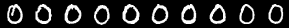
\includegraphics[width=0.9\linewidth]{predoc/images/0_ppv.png}\\
  
\includegraphics[width=0.90\linewidth]{predoc/images/1_ppv.png}\\
  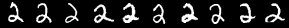
\includegraphics[width=0.90\linewidth]{predoc/images/2_ppv.png}\\
  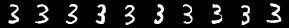
\includegraphics[width=0.90\linewidth]{predoc/images/3_ppv.png}\\
  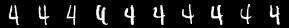
\includegraphics[width=0.90\linewidth]{predoc/images/4_ppv.png}\\
  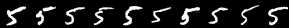
\includegraphics[width=0.90\linewidth]{predoc/images/5_ppv.png}\\
  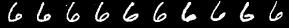
\includegraphics[width=0.90\linewidth]{predoc/images/6_ppv.png}\\
  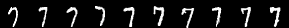
\includegraphics[width=0.90\linewidth]{predoc/images/7_ppv.png}\\
  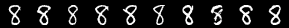
\includegraphics[width=0.90\linewidth]{predoc/images/8_ppv.png}\\
  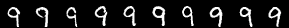
\includegraphics[width=0.90\linewidth]{predoc/images/9_ppv.png}
\end{tabular}
\label{fig:mnistppv}
\end{subfigure}
\begin{subfigure}{0.45\textwidth}
% \subfigure[$10$-pca components]{
\begin{tabular}{c}
  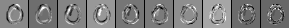
\includegraphics[width=0.9\linewidth]{predoc/images/0_eigenvectors.png}\\
  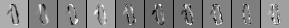
\includegraphics[width=0.90\linewidth]{predoc/images/1_eigenvectors.png}\\
  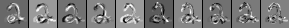
\includegraphics[width=0.90\linewidth]{predoc/images/2_eigenvectors.png}\\
  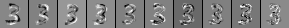
\includegraphics[width=0.90\linewidth]{predoc/images/3_eigenvectors.png}\\
  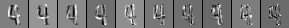
\includegraphics[width=0.90\linewidth]{predoc/images/4_eigenvectors.png}\\
  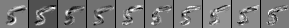
\includegraphics[width=0.90\linewidth]{predoc/images/5_eigenvectors.png}\\
  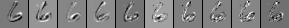
\includegraphics[width=0.90\linewidth]{predoc/images/6_eigenvectors.png}\\
  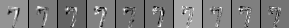
\includegraphics[width=0.90\linewidth]{predoc/images/7_eigenvectors.png}\\
  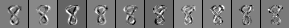
\includegraphics[width=0.90\linewidth]{predoc/images/8_eigenvectors.png}\\
  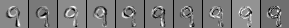
\includegraphics[width=0.90\linewidth]{predoc/images/9_eigenvectors.png}
\end{tabular}
\label{fig:mnistpca}
\end{subfigure}

   \caption{Sur MNIST, pour un exemple de chaque classe (chiffres de $0$ à $9$) on
   extrait les $10$ plus proches voisins (ppv) intra-classe et on entraîne une PCA sur cet
   ensemble. Les $10$ ppv sont présentés en Fig.~\ref{fig:mnistppv} et les
   composantes des $10$ différentes PCA en Fig.~\ref{fig:mnistpca}. Les premières composantes de
   la PCA contiennent des informations utiles (de possibles transformations)
   tandis que les dernières n'encodent que du bruit.}

\end{figure}


On s'intéresse ici à des méthodes qui peuvent être utilisées par la suite pour
l'initialisation de réseaux de neurones.
%(voir Section~\ref{sec:nn})
Depuis la formalisation la plus classique de l'auto-encodeur
\textbf{(AE)}~\cite{Gallinari87} , nous présenterons le \textit{Denoising
Auto-Encoder} \textbf{(DAE)}~\cite{VincentPLarochelleH2008,Vincent-JMLR-2010}.
%Après une analyse de l'effet du bruit utilisée lors du processus
%d'apprentissage,
Ensuite, nous présenterons le \textit{Contractive Auto-Encoder}
\textbf{(CAE)}~\cite{Rifai+al-2011,Salah+al-2011} et sa version la plus
sophistiquée le \textit{Higher-Order Contractive Auto-Encoder}
\textbf{(CAE+H)}~\cite{Salah+al-2011}.

\subsection{Architectures de type Auto-Encodeur}

L'auto-encodeur classique se décompose en un encodeur et un décodeur.
L'encodeur effectue une transformation affine des données paramétrisée par une
matrice de poids $W\in\mathcal{M}_{m\times d}(\mathbb{R})$ où $m$ désigne le
nombre d'unités cachées du modèle et un vecteur de biais $b\in\mathbb{R}^m$.
Cette transformation est suivie d'une non-linéarité $s:\mathbb{R}^m \rightarrow
\mathbb{R}^m$ appliquée à chaque élément du vecteur. En général, on utilise la
fonction logistique $s(x)=1/(1+e^{-x})$ mais la tangente hyperbolique est aussi
communément utilisée. On a donc la forme globale suivante:

\begin{equation}
h(x)=s(Wx+b)
\end{equation}

Le décodeur tente de reconstruire l'exemple $x$ à partir de la représentation
cachée $h(x)$ et peut partager en la m\^eme matrice de poids que l'encodeur
mais a un vecteur de biais $b^{'}\in\mathbb{R}^d$ qui lui est propre. Il a
alors la forme suivante:

\begin{equation}
r(x)=s(W^{T} h(x)+b^{'})
\end{equation} 

La non-linéarité $s(.)$ est ici optionnelle et dépend de la nature des données
ou de la sortie désirée du décodeur \textit{i.e.} si elle doit \^etre dans
l'intervalle $[0,1]$ ou non.  \\

\paragraph{Algorithme}
Tous ces paramètres sont ajustés par optimisation \textit{e.g.} descente de
gradient stochastique, visant à réduire l'erreur de reconstruction suivante:

\begin{equation}
\mathcal{J}_{\textrm{AE}} = \frac{1}{\vert \mathcal{D}\vert}\sum_{x\in\mathcal{D}}\mathcal{L}(x,r(h(x)))
\label{eq:ae}
\end{equation}

La fonction de perte $\mathcal{L}$ utilisée est en général, dans le cas de
données binaires (ou modélisant des probabilités), l'entropie croisée négative
$\mathcal{L}(x,y) = -\sum_{i=1}^d x_i\log y_i + (1-x_i)\log(1-y_i)$ ou la
\textit{Mean Squared Error} (MSE) $\mathcal{L}(x,y) = \| x-y\|^2_2$. Comme on
le verra par la suite à la Section~\ref{sec:perfs}, pour les fins
d'initialisation de réseaux de neurones de classification, les performances de
l'auto-encodeur classique sont largement dépassées par le DAE, CAE et CAE+H.

\paragraph{Hyperparamètres} Les hyperparamètres de ce genre d'architecture sont
malheureusement nombreux. En voici une liste non exhaustive et des exemples de
valeurs typiques à raffiner par une recherche des hyperparamètres optimaux: le
nombre d'unités cachées ($1,000$), la fonction d'activation de l'encodeur ou et
du décodeur (fonction sigmoide), la fonction de perte utilisée (MSE ou Entropie
croisée), le pas de gradient ($\lbrace 10^{-1},\dots,10^{-6}\rbrace$).  \\

Une fois une certaine expertise pratique acquise avec l'entraînement de ce genre
d'architectures, l'espace des hyperparamètres à explorer qui peut paraître
exponentiellement grand au premier abord peut se réduire à quelques valeurs.


\subsubsection{Auto-Encodeur Débruitant}

On présente ici l'Auto-Encodeur Débruitant, en anglais \textit{Denoising
Auto-Encoder} (DAE).  L'idée du DAE est qu'à partir de l'observation partielle
d'une entrée on doit être capable de reconnaître (reconstruire) l'entrée
originale. À un très haut niveau, on peut penser qu'en tant qu'êtres humains,
nous sommes capables de reconnaître des objets partiellement occultés ou aussi
bien à partir d'un son et d'une image, nous sommes en mesure de reconnaître un
film déjà vu en ne voyant que certaines séquences.  \\

Plutôt que de minimiser la perte classique Eq.~\ref{eq:ae}, on bruite l'entrée
$x$ et on force l'auto-encodeur à reconstruire l'entrée originale à partir de
la version bruitée $\tilde{x}$:

\begin{equation}
\mathcal{J}_{\textrm{DAE}} = \frac{1}{\vert \mathcal{D}\vert}\sum_{x\in\mathcal{D}}\mathcal{L}(x,r(h(\tilde{x})))
\label{eq:dae}
\end{equation}

Les processus de corruption communément utilisés sont le \textit{masking}
paramétré par $p$ la probabilité de mettre à zéro une composante de l'entrée ou
le bruit gaussien paramétré par $\sigma$ où $\tilde{x} = x + \epsilon$ où
$\epsilon \sim \mathcal{N}(0,\sigma)$. D'autres types de bruit
peuvent être utilisés (voir \cite{Vincent-JMLR-2010} pour une revue).

\paragraph{Hyperparamètres} On peut citer ici en plus des hyperparamètres de
l'auto-encodeur classique le type de bruit (gaussien ou \textit{masking}) et le niveau
de bruit.

%\section{Analyse de l'effet du bruit au cours de l'apprentissage}

%Différence entre DAE et CAE. Le DAE va avoir un décodeur qui est invariant à de
%petites variations de l'entrée. Sachant que seul l'encodeur est conservé pour
%l'entraînement de réseaux de neurones, il serait préférable d'avoir le encodeur
%qui soit invariant (CAE) et non pas le décodeur (DAE). 

\subsubsection{Auto-Encodeur Contractant}

On présente ici l'Auto-Encodeur Contractant, en anglais \textit{Contractive
Auto-Encoder}.
Contrairement à la PCA qui extrait les directions de variations
\textbf{globales} présente dans les exemples d'apprentissage, le CAE apprend
des directions de variations \textbf{locales}. Il suffit d'ajouter de manière
explicite dans la perte minimisée Eq.~\ref{eq:ae} une régularisation qui
correspond à la norme du jacobien de l'encodeur $h(x)$ par rapport à l'entrée
$x$ sur les points de l'ensemble d'entraînement $\mathcal{D}$:

\begin{equation}
\mathcal{J}_\textrm{CAE} = \mathcal{J}_\textrm{AE} + \lambda\frac{1}{\vert \mathcal{D}\vert}\sum_{x\in\mathcal{D}}\| \frac{\partial h}{\partial x}(x)\|_2^2
\label{eq:cae}
\end{equation}

Cette approche suggère aussi la possibilité de visualiser dans l'espace
d'entrée quelles sont les directions de variation autour d'un exemple
d'apprentissage auxquelles la représentation $h$ est sensible  (en regardant
les vecteurs propres du jacobien au point d'apprentissage). Cela permet
d'évaluer d'un point de vue qualitatif si l'extraction de caractéristiques a
convergé vers une solution intéressante ou non (voir Figure~\ref{fig:tan}).

\paragraph{Hyperparamètres} Contrairement au DAE, le CAE n'a ici qu'un seul
hyperparamètre en plus comparé à l'auto-encodeur classique. C'est le
coefficient de régularisation $\lambda$ ($0.1$ est un bon point de départ pour
chercher le coefficient optimal) qui va contrôler le compromis entre
erreur de reconstruction et invariance de la représentation.

\begin{figure}
\centering
\begin{subfigure}{0.9\linewidth}
%\subfigure[composantes d'une PCA sur CIFAR]
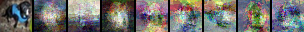
\includegraphics[width=0.9\linewidth]{predoc/images/pca.png}
\label{fig:tan_pca}
\end{subfigure}

\begin{subfigure}{0.9\linewidth}
%\subfigure[tangentes du CAE+H sur CIFAR]
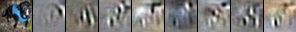
\includegraphics[width=0.9\linewidth]{predoc/images/tangents_cifar.png}
\label{fig:tan_cifar}
\end{subfigure}

\begin{subfigure}{0.9\linewidth}
%\subfigure[tangentes du CAE+H sur MNIST]
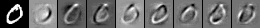
\includegraphics[width=0.9\linewidth]{predoc/images/tangents_mnist.png}
\label{fig:tan_mnist}
\end{subfigure}


   \caption{ Sur MNIST et sur CIFAR (un ensemble d'predoc/images RGB), on présente les
   tangentes apprises par le CAE+H autour d'un point d'apprentissage en
   Figure~\ref{fig:tan_mnist},\ref{fig:tan_cifar}. On peut voir que ces
   tangentes encodent de l'information sur des transformation plausibles de
   l'image originale tandis que les composantes principales de la PCA n'ont
   encodé que du bruit (voir Figure~\ref{fig:tan_pca}). 
\label{fig:tan}}

\end{figure}





\subsubsection{Auto-Encodeur Contractant d'Ordre Supérieur}

Nous présentons ici une publication qui s'inscrit dans la recherche à laquelle j'ai contribué
au cours de mes deux premières années de doctorat \cite{Salah+al-2011}: il s'agit
de l'auto-encodeur contractant d'ordre supérieur, en anglais
\textit{Higher-order Contractive Auto-Encoder} (CAE+H).


Si le fait de pénaliser le premier ordre de la dérivée (jacobien) de l'encodeur
par rapport à l'entrée est bénéfique, il est naturel d'ajouter une pénalisation
concernant les ordres supérieurs (Hessien, troisième ordre, ...) au CAE
original (Eq.~\ref{eq:cae}). On pourra alors constater les effets obtenus en
termes de mesures quantitatives de performances de classification (bénéfique ou
non) ou de directions de variations obtenues (qualitatif).

Les pertes Eq.~\ref{eq:ae},~\ref{eq:dae} ou~\ref{eq:cae} sont minimisées par
descente de gradient. Il est donc nécessaire de pouvoir calculer les dérivées
partielles de la perte par rapport aux paramètres. Pour commencer, le calcul de
la $k^{\textrm{ième}}$ dérivée de l'encodeur (avec $m$ unités cachées) par
rapport à l'entrée (de dimension $d$) a une complexité algorithmique de
$O(md^k)$.  Calculer les dérivées partielles de cette dérivée par rapport aux
paramètres du modèles est donc prohibitif. Pour éviter ce calcul, on utilise
une approximation stochastique de la Hessienne (voir \cite{Salah+al-2011} pour
la preuve):

\begin{equation}
\|\dfrac{\partial^2 h}{\partial x^2}(x) \|_2^2 = \lim_{\sigma\rightarrow 0}\frac{1}{\sigma^2}\int_{\epsilon \rightsquigarrow \mathcal{N}(0,\sigma)} \| \dfrac{\partial h}{\partial x}(x) - \dfrac{\partial h}{\partial x}(x+\epsilon) \|^2_2 d\epsilon
\label{eq:hessian-approx}
\end{equation}

Si la variance $\sigma$ est non nulle, des contributions aux normes des ordres
supérieurs apparaissent \cite{Salah+al-2011}. Ces contributions disparaissent à
la limite $\sigma\rightarrow 0$. En pratique pour approximer la norme de la
Hessienne (Eq.~\ref{eq:hessian-approx}), on utilise un lot de plusieurs
versions bruitées $x+\epsilon$ du m\^eme exemple $x$ avec un $\sigma$ petit
mais non négligeable, ce qui donne lieu à l'approximation stochastique de la
norme de la Hessienne qui comporte aussi d'autres contributions provenant des
normes des ordres supérieurs (voir \cite{Salah+al-2011} pour plus de détails).

L'avantage d'utiliser cette approximation est que l'on peut pénaliser tous les
ordres supérieurs à moindre coût comparé à une complexité en $O(md^k)$.
L'inconvénient est de ne plus savoir exactement quels ordres sont pénalisés et
quelle est la contribution de chacun des ordres qui permet d'apprendre de
meilleures caractéristiques. Des expériences supplémentaires seront effectuées
sur des données de dimension réduite afin d'améliorer notre compréhension du
CAE+H.

En utilisant cette approximation,  on aboutit à la perte du \textbf{CAE+H} avec
une taille de lot $n_c$ et $\epsilon_i \rightsquigarrow \mathcal{N}(0,\sigma)$:

\begin{equation}
\mathcal{J}_\textrm{CAE+H} = \mathcal{J}_\textrm{CAE} + \gamma\frac{1}{\vert \mathcal{D}\vert}\sum_{x\in\mathcal{D}} \frac{1}{n_c}\sum^{n_c}_{i=1} \| \dfrac{\partial h}{\partial x}(x) - \dfrac{\partial h}{\partial x}(x+\epsilon_i) \|^2_2 
\label{eq:cae}
\end{equation}

\paragraph{Hyperparamètres} Le problème du CAE+H est bien son nombre
d'hyperparamètres. En plus des hyperparamètres du CAE, on a ici le coefficient
de régularisation pour les ordres supérieurs $\gamma$, le niveau de bruit
gaussien $\sigma$ et la taille du mini-lot $n_c$ utilisés pour l'estimation de
la norme de la Hessienne.

\subsubsection{Autres Méthodes d'Extraction de Caractéristiques}

Il existe de nombreuses autres méthodes d'extraction de caractéristiques qui
n'ont pas été détaillées ici. En méthodes d'extraction de
caractéristiques linéaires, on trouve par exemple l'analyse en composantes
indépendantes, en anglais \textit{Independent Component Analysis}~\cite{Comon94,Hyvarinen-2001}. Cette
méthode peut être utilisée pour la séparation aveugle de sources.
\\

Deux types de méthodes d'extraction de caractéristiques non-linéaire  ont aussi
fait l'objet de récentes avancées: les méthodes {\bf sparses}
\cite{ranzato-08,koray-psd-08,Koray-08} qui utilisent une pénalité sur les
activations de l'encodeur (afin de le pousser à prendre les valeurs $1$ - actif
- ou $0$ - inactif - dans le cas d'une sigmoide)  ou les modèles {\bf
génératifs} basés sur des fonctions d'énergie \cite{ranzato-unsup-07} comme les
Machines de Boltzmann Restreintes, en anglais \textit{Restricted Boltzmann
Machine} \cite{Tieleman08}.  Ces méthodes ont été utilisées avec succès pour
l'initialisation de réseaux de neurones de type Perceptron Multi-Couches
\cite{HintonG2006,ranzato-08,koray-psd-08,Koray-08} ou Réseaux convolutionnels
\cite{koray-nips-10-small}.  Tout en nous concentrant sur les variantes
d'auto-encodeurs que nous venons de présenter, nous considèrerons notamment
aussi les RBMs comme point de référence dans les évaluations de performances
quantitatives qui suivent.

\subsection{Déplacement sur la Variété}

Relire le papier MTC

En observant les vecteurs propres d une pca calculee sur un ensemble de points
voisins, une similitude a ete observee avec des potentielles directions de
variations autour de ce point. L'idee est qu'il est possible d'avoir un
ensemble de directions de variation pour chaque point de l'ensemble
d'Apprentissage. Il est possible de se deplacer sur la variet d'un point
d'entrainement a un  autre en suivants ces directions.

Cette idee de deplacemet (cite Surfing on the manifold) plus aisee dans des
couches de representations plus abstraites et notamment d'une classe a un autre
classe differente est l'intuition derriere la possibilite d'avoir un meilleur
mixing lors du processus de sampling utilise avec des CAE ou des RBM.

\subsection{Transfert de Domaine}


intro du transfert de domaine basee sur le pere grolot

\subsubsection{Transductive PCA}
\subsubsection{Finetuning}


\section{Classification de Séquences}

prédiction séquentielle

\subsection{Conditionnal Random Fields}


\subsection{Reseaux de Neurones Recurrents}


